\documentclass[11pt,a4paper]{article}

\usepackage[polish]{babel}
\usepackage[utf8]{inputenc}
\usepackage{polski}
\usepackage[T1]{fontenc}
\usepackage{indentfirst}
\usepackage{wrapfig}    % for wrapping figures, tables

\frenchspacing

%\usepackage{amsmath}
\usepackage{physics}
%\usepackage{bm}
\usepackage{gensymb}
%\usepackage{hepnames}
\usepackage{epsfig}
\usepackage{graphics}
\usepackage[shortlabels]{enumitem}
%\usepackage{xspace}
%\xspaceaddexceptions{[]\{\}}

%
%
%fixpagesize
\pagestyle{empty}
\addtolength{\textwidth}{6cm}
\addtolength{\textheight}{4cm}
\addtolength{\evensidemargin}{-3cm}
\addtolength{\oddsidemargin}{-3cm}
\addtolength{\topmargin}{-2cm}
\parindent=0cm


%
%
%small distance in list/item/enum for enumitem package
\setlist[itemize,enumerate]{topsep=0em}
\setlist{noitemsep}

%print zadanie #
\newcounter{zadanie}\newcommand{\zadanie}[1][]{\addtocounter{zadanie}{1} ~\\  {\bf \emph{Zadanie \arabic{zadanie} #1 }} \\}
\newcounter{zaddom}\newcommand{\zaddom}[1][]{\addtocounter{zaddom}{1} ~\\  {\bf \emph{Zadanie domowe \arabic{zaddom} #1 }} \\}
%\renewcommand{\zadanie}[1][]{\pagebreak  ~\\  {\bf \emph{Zadanie }} \\} \addtolength{\topmargin}{-2cm}

\newcommand{\dbar}{{\mkern3mu\mathchar'26\mkern-12mu d}}


%%%%%%%%%%%%%%%%%%%%%%%%%%%%%%%%%%%%%%%%%%%%%%%%%%%%%%
\begin{document}           % End of preamble and beginning of text.

\begin{centering}
\bf{\Large{Termodynamika z elementami fizyki statystycznej}}\\
Tydzień 7 (17 kwietnia 2023)\\[3mm]
Cykle termodynamiczne, maszyny cieplne\\
\end{centering} 
\vspace{5mm}

\zadanie
Dla teoretycznej maszyny cieplnej, której gazem roboczym jest gaz doskonały, 
i pracującej w oparciu o cykl Carnota, znajdź bezpośrednim rachunkiem:
\begin{enumerate}[a)]
\item sprawność silnika
\item efektywność lodówki
\item efektywność pompy cieplnej
\end{enumerate}
Załóź, że maszyna działa między dwoma zbiornikami o temperaturach 0\degree C i 60\degree C.

\begin{wrapfigure}[10]{r}{0.3\linewidth}\vspace{0mm}
\resizebox{\linewidth}{!}{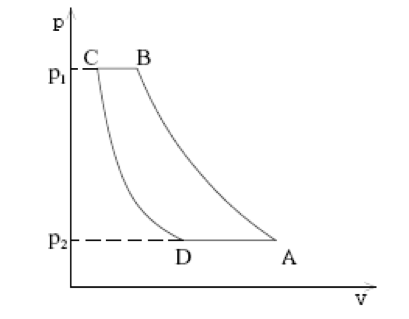
\includegraphics{rys_lodowa.png}}
\end{wrapfigure}
\zadanie
Zbudowano lodówkę działającą w następującym procesie cyklicznym (rysunek): gaz roboczy jest najpierw sprężany izotermicznie w temperaturze otoczenia $T_1$ do ciśnienia $p_1$. Sprężony gaz doprowadzany jest do kontaktu termicznego z wnętrzem lodówki i chłodzony izobarycznie do jego temperatury $T_2$. Następnie, wciąż w kontakcie z wnętrzem lodówki, gaz jest izotermicznie rozprężany do ciśnienia $p_2$. Wreszcie doprowadzany jest z powrotem do kontaktu termicznego z otoczeniem i ogrzewa się izobarycznie do temperatury $T_1$, powracając w ten sposób do stanu początkowego.
Przyjmując, że gaz roboczy jest dwuatomowym gazem doskonałym ($C_p=\frac{7}{2}R$):
\begin{enumerate}
\item Znajdź współczynnik sprawności opisanej lodówki.
\item Oblicz, dla jakiej najniższej temperatury $T_2$ lodówka będzie jeszcze działać przy ustalonych $T_1, p_1$ i $p_2$ (tzn. będzie jeszcze pobierała ciepło ze swego wnętrza).
\end{enumerate}

\begin{wrapfigure}[10]{r}{0.3\linewidth}\vspace{-5mm}
\resizebox{\linewidth}{!}{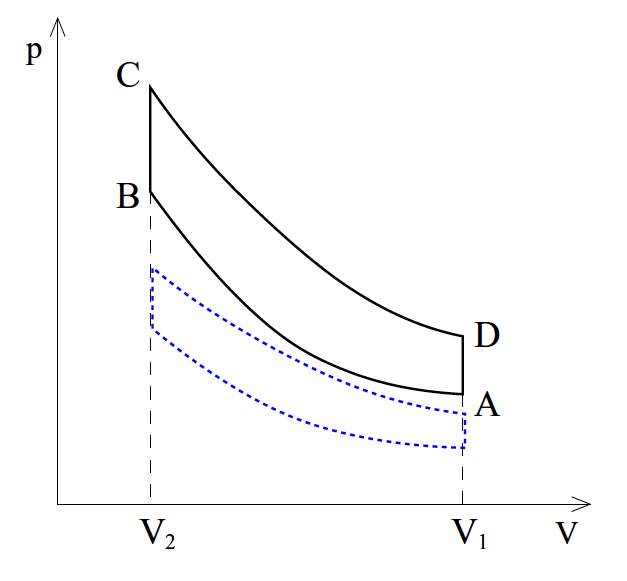
\includegraphics{rys_otto.png}}
\end{wrapfigure}
\zadanie
Działanie silnika spalinowego można w przybliżeniu opisać tzw. cyklem
Otto (rysunek). W cyklu tym gaz wypełniający cylinder (mieszanka powietrza z paliwem,
pobrana w cyklu ssania) jest najpierw adiabatycznie sprężany od objętości $V_1$
do $V_2$. W chwili osiągnięcia minimalnej objętości mieszanka jest zapalana. Wydzielone ciepło
powoduje izochoryczny wzrost ciśnienia gazu. Następuje adiabatyczne rozprężenie z powrotem
do objętości początkowej $V_1$. W punkcie tym otwierany jest zawór wydechowy.
Rozprężanie gazu powoduje spadek temperatury. Oblicz sprawność takiego silnika.

\zadanie
Rozważyć proces cykliczny w którym gaz doskonały najpierw jest izotermicznie rozprężany 
do próżni od objętości $V_A$ do $V_B$, 
następnie izobarycznie ($p=p_0=const$) jest sprężany do objętości $V_A$, 
po czym ogrzewany jest on izochorycznie ($V=V_A=const$) tak, 
iż stan układu wraca do stanu początkowego. 
Jest to cykl Mayera i za jego pomocą wykaż dla gazu doskonałego, że $C_p-C_v=R$.

\zadanie
Znajdź sprawność silnika, który działa w oparciu o cykl Carnota między temperaturami 
$T_2$ i $T_1$ ($T_2<T_1$) i w którym substancją roboczą jest gaz fotonowy.

\pagebreak
~
\zaddom
Cykl termodynamiczny $n$ moli gazu doskonałego składa się z dwóch izoterm o temperaturach $T_1$ i $T_2$
 (przy czym $T_1 > T_2$) i z dwóch izobar odpowiadających ciśnieniom $p_1$ i $p_2$ ($p_1 > p_2$).
 Oblicz sprawność silnika działającego w oparciu o taki cykl.

\begin{wrapfigure}[8]{r}{0.25\linewidth}\vspace{-5mm}
\resizebox{\linewidth}{!}{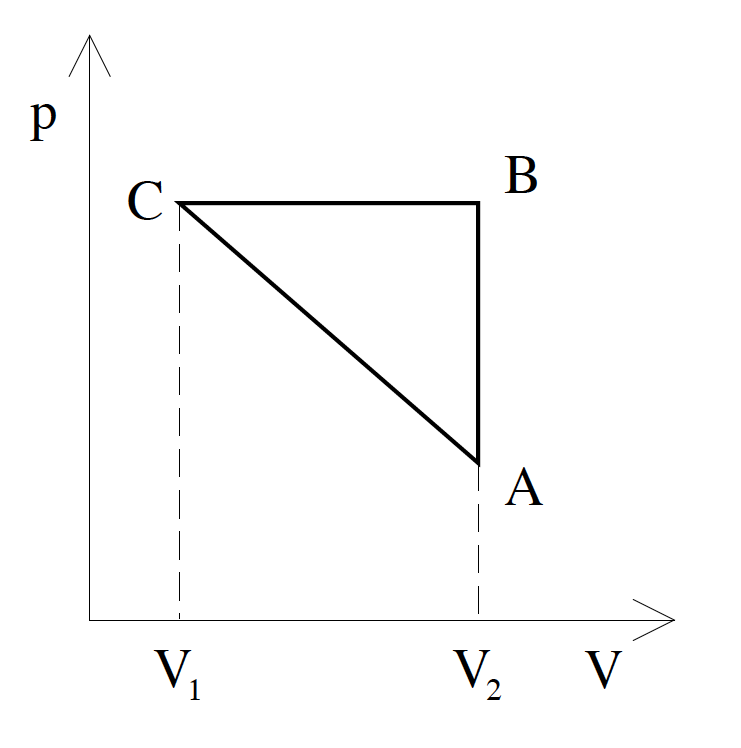
\includegraphics{seria2_rys3.png}}
\end{wrapfigure}
\zaddom
Lodówka, w której ciałem roboczym jest gaz doskonały
o cieple molowym $C_V=\frac{3}{2} R$, pracuje w cyklu przedstawionym na rysunku.
W fazie izochorycznego wzrostu ciśnienia gaz roboczy wymienia ciepło
z wnętrzem lodówki, a w pozostałych fazach wymienia ciepło z otoczeniem.
Proces $BC$ jest opisywany linią prostą we współrzędnych $p-V$.
Oblicz sprawność lodówki.

%~\vspace*{1cm}
% 
%\begin{wrapfigure}[6]{r}{0.25\linewidth}\vspace{-5mm}
%\resizebox{\linewidth}{!}{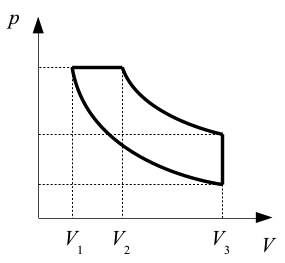
\includegraphics{seria2_rys5.png}}
%\end{wrapfigure}
%\zaddom
%Idealny silnik cieplny pracuje w cyklu Diesla (tj. dwie adiabaty, jedna izobara, jedna izochora),
%którego kontur we współrzędnych $p-V$ przedstawiony jest na rysunku.
%Zaznacz właściwy kierunek cyklu.
%Wyraź sprawność silnika przez stosunki objętości $V_1$, $V_2$, $V_3$.
%Substancją roboczą jest gaz doskonały o cieple molowym $C_V$.\\[1mm]
%
%~\vspace*{1cm}
%
%\begin{wrapfigure}[6]{r}{0.275\linewidth}\vspace{-5mm}
%\resizebox{\linewidth}{!}{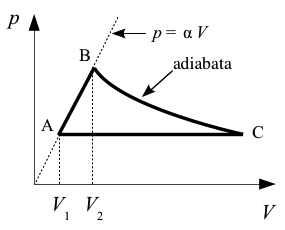
\includegraphics{seria2_rys6.png}}
%\end{wrapfigure}
%\zaddom
%Oblicz sprawność idealnego silnika cieplnego pracującego w cyklu przedstawionym
%na rysunku i wyraź ją poprzez wielkości: $\alpha$, $V_1$ i $V_2$.
%Odcinek $AB$ jest linią prostą o nachyleniu $\alpha$, zaś $BC$ jest adiabatą.
%Przyjmij, że ciałem roboczym jest jednoatomowy gaz doskonały.
%Oblicz zmianę entropii na odcinku $AB$.\\

~\vspace*{1cm}

\begin{wrapfigure}[6]{r}{0.3\linewidth}\vspace{0mm}
\resizebox{\linewidth}{!}{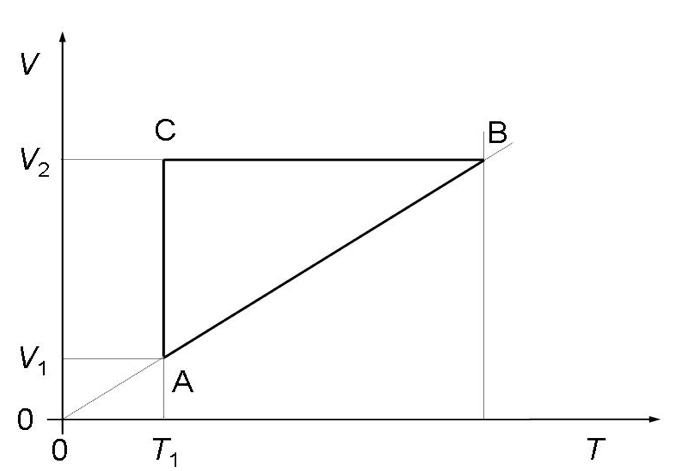
\includegraphics{seria2_rys7.png}}
\end{wrapfigure}
\zaddom
Jeden mol jednoatomowego gazu doskonałego podlega przemianom
cyklicznym przedstawionym we współrzędnych $V-T$ na rysunku obok.
Narysuj ten cykl we współrzędnych $p-V$ i oblicz sprawność
idealnego silnika cieplnego pracującego w takim cyklu.
Dane są: $T_1$, $V_1$, $V_2$.\\[1mm]


\pagebreak

\begin{centering}
\bf{ Odpowiedzi do zadań domowych }\\[1mm]
\end{centering}
\vspace{1mm}

\setcounter{zaddom}{0}

\zaddom
$\eta = \frac{R(T_1 - T_2) \ln p_1/p_2}{C_p(T_1 - T_2) + R T_1 \ln p_1/p_2}$.

\zaddom
$\eta = \frac{3 V_2}{V_2 - V_1}$.

\zaddom
$\eta = 1 - \frac{C_V}{C_P} \frac{V_3}{V_2 -V_1} \frac{V_2^{\kappa} - V_1^{\kappa}}{V_3^{\kappa}}$.



%\zaddom
% $\eta = 1 - \frac{C_p}{C_V + R/2} \frac{V_1 (V_1 - V_3)}{V_2^2 - V_1^2}$, gdzie $V_3 = V_2 (V_2/V_1)^{1/\kappa}$.
%$\Delta S_{AB} = n C_p \ln V_3/V_1$. 
%
%\zaddom
% $\eta = 1 - \frac{C_V}{C_p} - \frac{R \ln V_2/V_1}{C_p(V_2/V_1 - 1)}$.

% An example of figure placement:
%\begin{wrapfigure}[13]{r}{0.4\linewidth}\vspace{3mm}
%\resizebox{\linewidth}{!}{\includegraphics{NAZWA.png}}
%\end{wrapfigure}
%\zadanie

\end{document}
\end{document}
